\documentclass{standalone}
%https://tex.stackexchange.com/questions/489712/stacking-3d-cubes-with-spacing
\usepackage{tikz}
\usetikzlibrary{3d}
\def\cx{.99} % relative size of cube vs grid unit
\newcommand{\cube}[4][black]{
  \fill[#1!30,opacity=0.8] (#2,#3,#4) -- (#2+\cx,#3,#4) -- (#2+\cx,#3+\cx,#4) -- (#2,#3+\cx,#4) -- cycle;
  \fill[#1!20,opacity=0.8] (#2,#3+\cx,#4) -- (#2,#3+\cx,#4-\cx) -- (#2+\cx,#3+\cx,#4-\cx) -- (#2+\cx,#3+\cx,#4) -- cycle;
  \fill[#1!40,opacity=0.8] (#2+\cx,#3,#4) -- (#2+\cx,#3+\cx,#4) -- (#2+\cx,#3+\cx,#4-\cx) -- (#2+\cx,#3,#4-\cx) -- cycle;
}

\newcommand{\widecube}[4][black]{
  \fill[#1!30,opacity=0.8] (#2,#3,#4) -- (#2+2*\cx,#3,#4) -- (#2+2*\cx,#3+\cx,#4) -- (#2,#3+\cx,#4) -- cycle;
  \fill[#1!20,opacity=0.8] (#2,#3+\cx,#4) -- (#2,#3+\cx,#4-\cx) -- (#2+2*\cx,#3+\cx,#4-\cx) -- (#2+2*\cx,#3+\cx,#4) -- cycle;
  \fill[#1!40,opacity=0.8] (#2+2*\cx,#3,#4) -- (#2+2*\cx,#3+\cx,#4) -- (#2+2*\cx,#3+\cx,#4-\cx) -- (#2+2*\cx,#3,#4-\cx) -- cycle;
}

\newcommand{\tallcube}[4][black]{
  \fill[#1!30,opacity=0.8] (#2,#3,#4) -- (#2+\cx,#3,#4) -- (#2+\cx,#3+2*\cx,#4) -- (#2,#3+2*\cx,#4) -- cycle;
  \fill[#1!20,opacity=0.8] (#2,#3+2*\cx,#4) -- (#2,#3+2*\cx,#4-\cx) -- (#2+\cx,#3+2*\cx,#4-\cx) -- (#2+\cx,#3+2*\cx,#4) -- cycle;
  \fill[#1!40,opacity=0.8] (#2+\cx,#3,#4) -- (#2+\cx,#3+2*\cx,#4) -- (#2+\cx,#3+2*\cx,#4-\cx) -- (#2+\cx,#3,#4-\cx) -- cycle;
}


\newcommand{\deepcube}[4][black]{
  \fill[#1!30,opacity=0.8] (#2,#3,#4) -- (#2+\cx,#3,#4) -- (#2+\cx,#3+\cx,#4) -- (#2,#3+\cx,#4) -- cycle;
  \fill[#1!20,opacity=0.8] (#2,#3+\cx,#4) -- (#2,#3+\cx,#4-2*\cx) -- (#2+\cx,#3+\cx,#4-2*\cx) -- (#2+\cx,#3+\cx,#4) -- cycle;
  \fill[#1!40,opacity=0.8] (#2+\cx,#3,#4) -- (#2+\cx,#3+\cx,#4) -- (#2+\cx,#3+\cx,#4-2*\cx) -- (#2+\cx,#3,#4-2*\cx) -- cycle;
}

\newcommand{\widetallcube}[4][black]{
  \fill[#1!30,opacity=0.8] (#2,#3,#4) -- (#2+2*\cx,#3,#4) -- (#2+2*\cx,#3+2*\cx,#4) -- (#2,#3+2*\cx,#4) -- cycle;
  \fill[#1!20,opacity=0.8] (#2,#3+2*\cx,#4) -- (#2,#3+2*\cx,#4-\cx) -- (#2+2*\cx,#3+2*\cx,#4-\cx) -- (#2+2*\cx,#3+2*\cx,#4) -- cycle;
  \fill[#1!40,opacity=0.8] (#2+2*\cx,#3,#4) -- (#2+2*\cx,#3+2*\cx,#4) -- (#2+2*\cx,#3+2*\cx,#4-\cx) -- (#2+2*\cx,#3,#4-\cx) -- cycle;
}

\newcommand{\widedeepcube}[4][black]{
  \fill[#1!30,opacity=0.8] (#2,#3,#4) -- (#2+2*\cx,#3,#4) -- (#2+2*\cx,#3+\cx,#4) -- (#2,#3+\cx,#4) -- cycle;
  \fill[#1!20,opacity=0.8] (#2,#3+\cx,#4) -- (#2,#3+\cx,#4-2*\cx) -- (#2+2*\cx,#3+\cx,#4-2*\cx) -- (#2+2*\cx,#3+\cx,#4) -- cycle;
  \fill[#1!40,opacity=0.8] (#2+2*\cx,#3,#4) -- (#2+2*\cx,#3+\cx,#4) -- (#2+2*\cx,#3+\cx,#4-2*\cx) -- (#2+2*\cx,#3,#4-2*\cx) -- cycle;
}

\newcommand{\talldeepcube}[4][black]{
  \fill[#1!30,opacity=0.8] (#2,#3,#4) -- (#2+\cx,#3,#4) -- (#2+\cx,#3+2*\cx,#4) -- (#2,#3+2*\cx,#4) -- cycle;
  \fill[#1!20,opacity=0.8] (#2,#3+2*\cx,#4) -- (#2,#3+2*\cx,#4-2*\cx) -- (#2+\cx,#3+2*\cx,#4-2*\cx) -- (#2+\cx,#3+2*\cx,#4) -- cycle;
  \fill[#1!40,opacity=0.8] (#2+\cx,#3,#4) -- (#2+\cx,#3+2*\cx,#4) -- (#2+\cx,#3+2*\cx,#4-2*\cx) -- (#2+\cx,#3,#4-2*\cx) -- cycle;
}
\pgfdeclareradialshading[tikz@ball]{ball}{\pgfqpoint{-20bp}{20bp}}{%
 color(0bp)=(tikz@ball!0!white);
 color(17bp)=(tikz@ball!0!white);
 color(21bp)=(tikz@ball!70!black);
 color(25bp)=(black!70);
 color(30bp)=(black!70)}
\makeatother

\newcommand{\boxcube}[3]{
  \draw (#1,#2,#3) -- (#1,#2+2,#3) -- (#1,#2+2,#3-2) -- (#1,#2,#3-2) -- (#1+2,#2,#3-2) -- (#1+2,#2+2,#3-2) -- (#1+2,#2+2,#3) -- (#1+2,#2,#3) -- cycle;
  \draw (#1,#2+2,#3) -- (#1+2,#2+2,#3);
  \draw (#1,#2+2,#3-2) -- (#1+2,#2+2,#3-2);
  \draw (#1,#2,#3) -- (#1,#2,#3-2);
  \draw (#1+2,#2,#3) -- (#1+2,#2,#3-2);
}

\definecolor{mygreen}{HTML}{118A4F}
\definecolor{myorange}{HTML}{DE6C06}
\definecolor{myviolet}{HTML}{8601AF}
% Positive Z-direction is out of the screen
\begin{document}
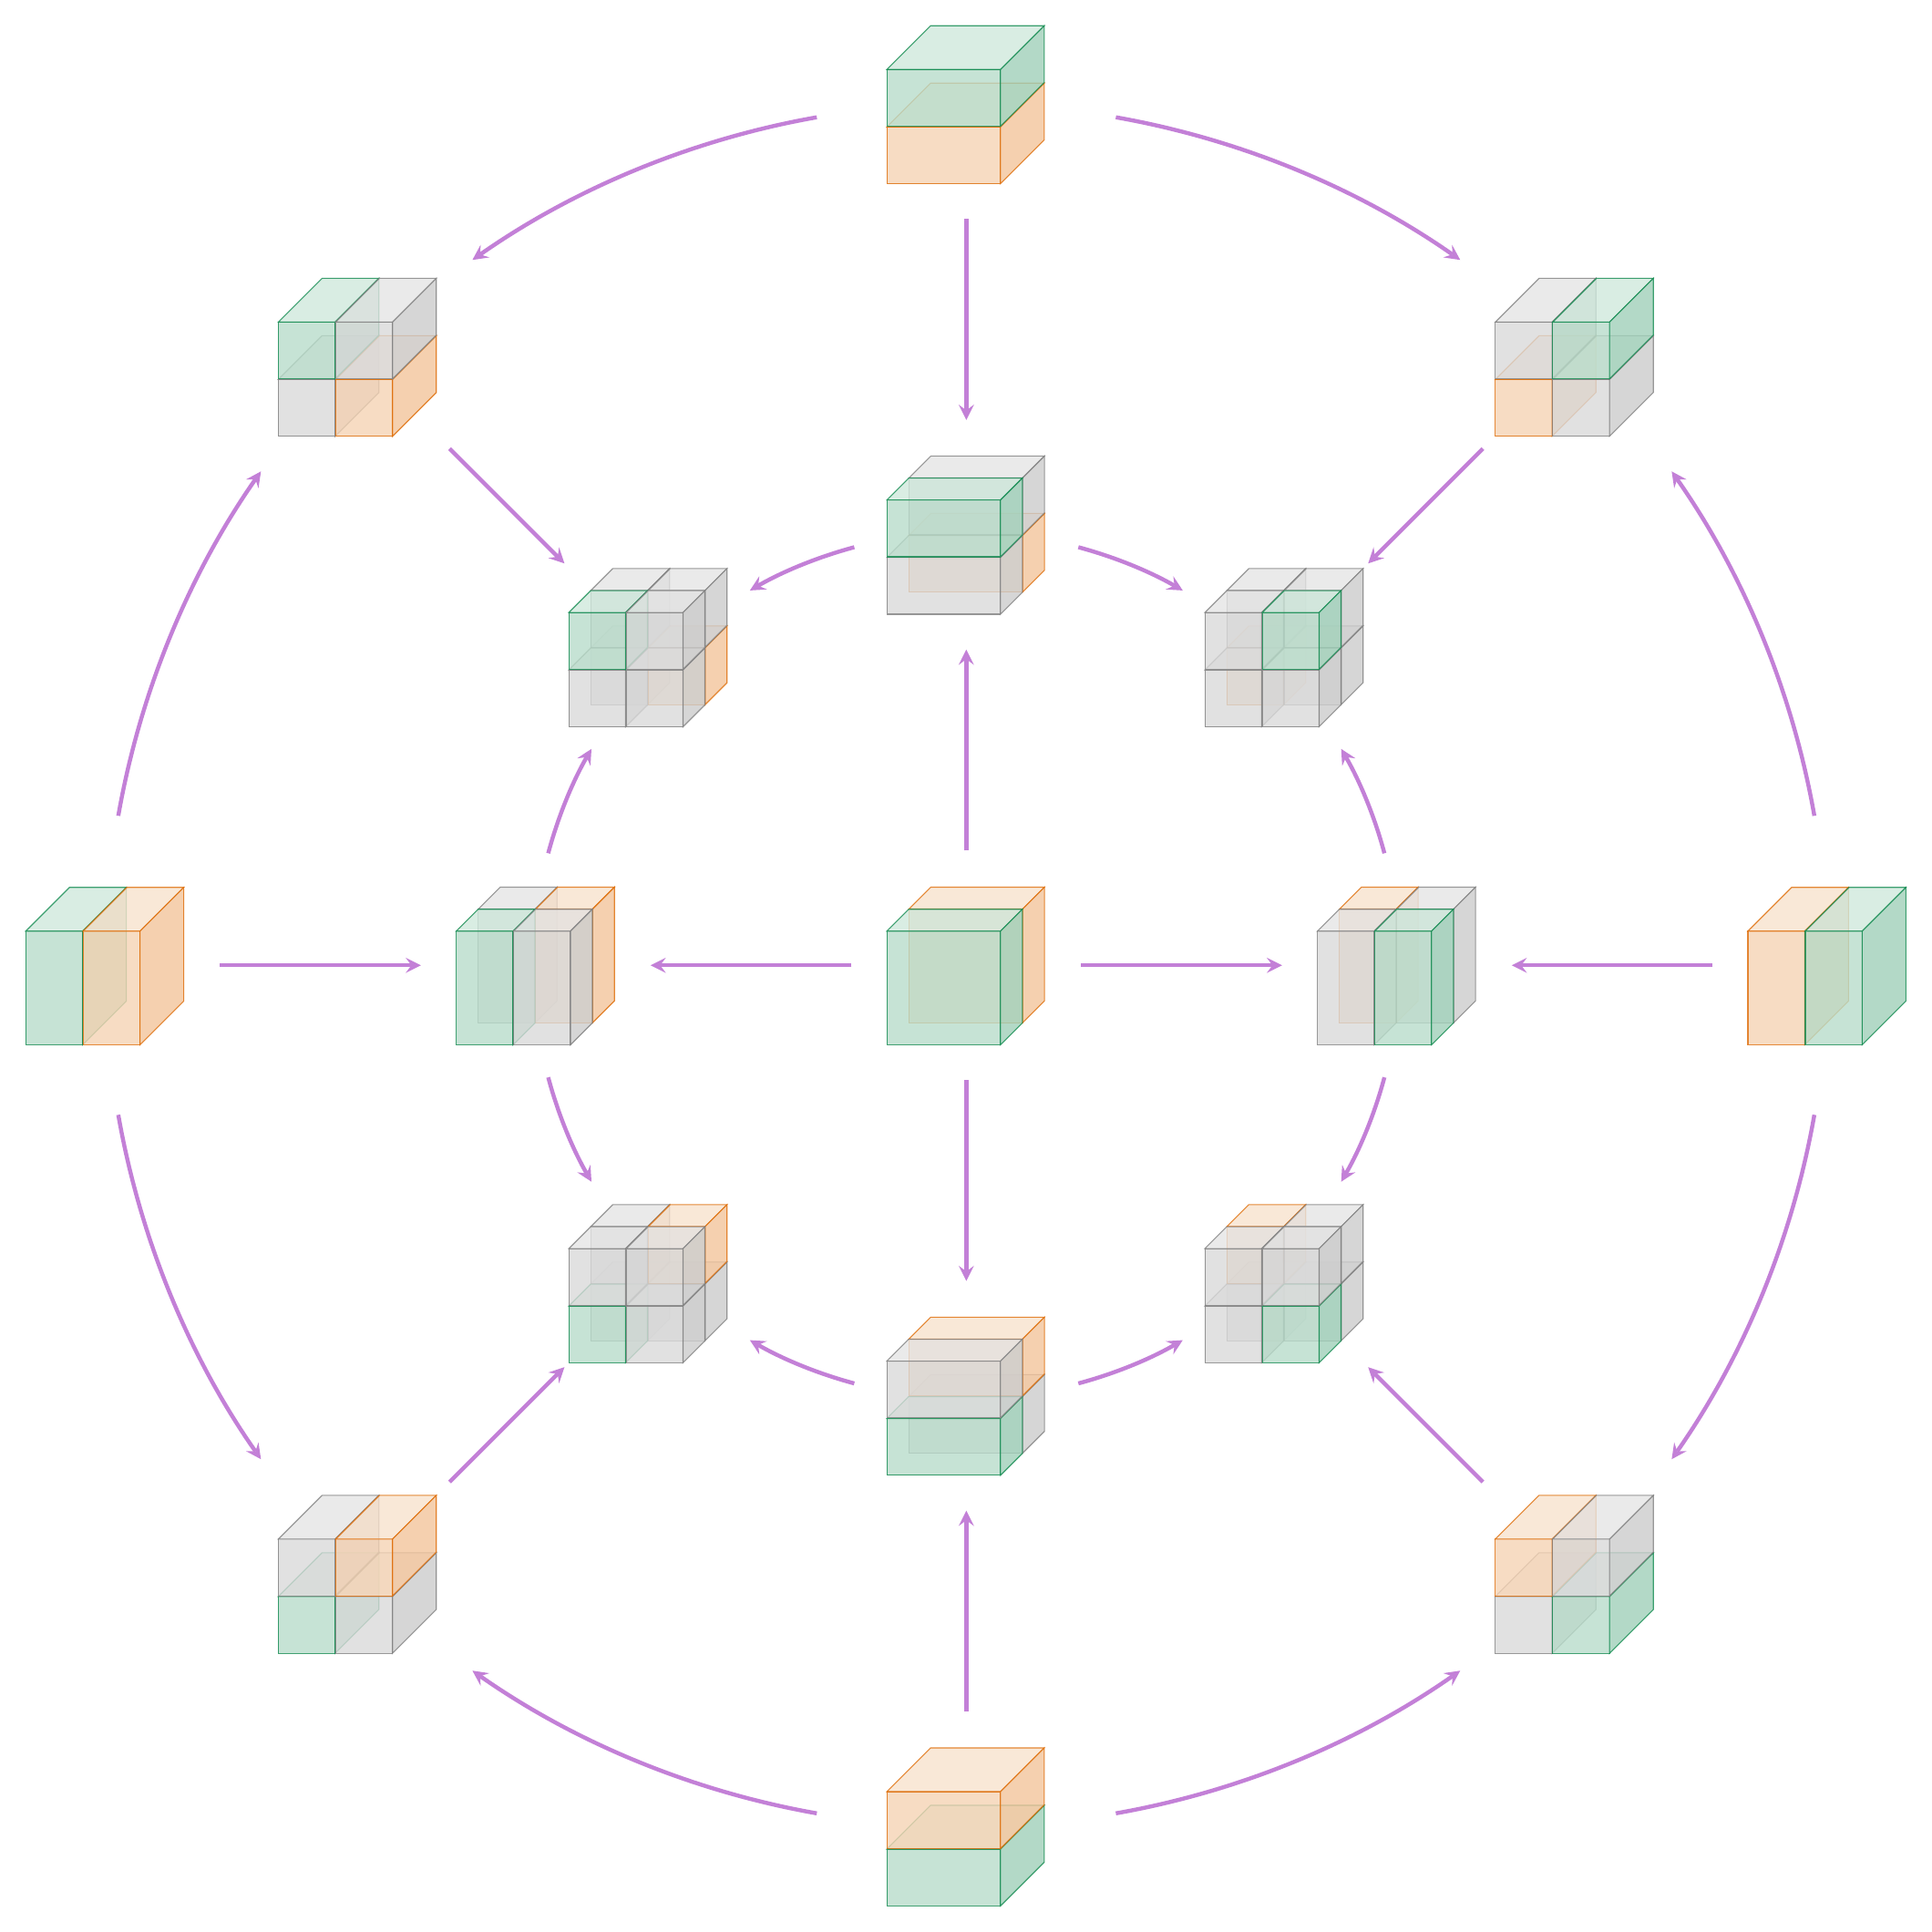
\begin{tikzpicture}[scale=0.8]

  % \foreach \ix in {1,2}{
  %   \foreach \iy in {1,2}{
  %     \foreach \iz in {1,2}{
  %       \cube[draw=mygreen,fill=mygreen]{\ix}{\iy}{\iz} }}}
  % \cube[draw=red,fill=red]{1}{2}{2}
  % \cube[draw=mygreen,fill=mygreen]{2}{2}{2}

  % \foreach \ix in {6,7}{
  %   \foreach \iy in {6,7}{
  %     \foreach \iz in {6,7}{
  %       \cube[draw=mygreen,fill=mygreen]{\ix}{\iy}{\iz} }}}

      % \begin{scope}
      %   \clip (11,0,0) circle (12);
      %   \shade [ball color=gray, opacity=0.2] (11,0,0) ellipse (11.2 and 11);
      % \end{scope}
  % \filldraw[opacity=0.1] (11,0,0) circle (10);
  % \draw[->] (1,1,0) -- (4,4,0);

  % \draw (0,0,0) -- (5,5,0) -- (10,10,0) -- (15,5,0) -- (20,0,0) -- (15,-5,0) -- (10,-10,0) -- (5,-5,0) -- (0,0,0);
  % \draw (0,0,0) -- (5,0,5) -- (10,0,10) -- (15,0,5) -- (20,0,0) -- (15,0,-5) -- (10,0,-10) -- (5,0,-5) -- (0,0,0);
  % \draw (10,0,10) -- (10,5,5) -- (10,10,0) -- (10,5,-5) -- (10,0,-10) -- (10,-5,-5) -- (10,-10,0) -- (10,-5,5) -- (10,0,10);

  %west pole
  % \cube[draw=myorange,fill=myorange]{0}{0.5}{-0.5}
  % \cube[draw=mygreen,fill=mygreen]{1}{0.5}{-0.5}
  % \draw[-] (0,-10) -- (0,10);
  % \draw[-] (-10,0) -- (10,0);
  % \draw[-] (0,0,-10) -- (0,0,10);  
  %Wpole
  \talldeepcube[draw=mygreen,fill=mygreen]{-16}{-1}{1}
  \talldeepcube[draw=myorange,fill=myorange]{-15}{-1}{1}

  %Npole
  \widedeepcube[draw=myorange,fill=myorange]{-1}{14}{1} 
  \widedeepcube[draw=mygreen,fill=mygreen]{-1}{15}{1}
   

  %Epole
  \talldeepcube[draw=myorange,fill=myorange]{14}{-1}{1}
  \talldeepcube[draw=mygreen,fill=mygreen]{15}{-1}{1}

  % %Spole
  \widedeepcube[draw=mygreen,fill=mygreen]{-1}{-16}{1} 
  \widedeepcube[draw=myorange,fill=myorange]{-1}{-15}{1}

  %center
  \widetallcube[draw=myorange,fill=myorange]{-1}{-1}{0}
  \widetallcube[draw=mygreen,fill=mygreen]{-1}{-1}{1}


  %middle left 
  % gray|orange
  % green|gray
  \tallcube[draw=gray,fill=gray]{-8.5}{-1}{0}
  \tallcube[draw=myorange,fill=myorange]{-7.5}{-1}{0}
  \tallcube[draw=mygreen,fill=mygreen]{-8.5}{-1}{1}
  \tallcube[draw=gray,fill=gray]{-7.5}{-1}{1}

  %middle right 
  % orange|gray
  % gray|green
  \tallcube[draw=myorange,fill=myorange]{6.5}{-1}{0}
  \tallcube[draw=gray,fill=gray]{7.5}{-1}{0}
  \tallcube[draw=gray,fill=gray]{6.5}{-1}{1}
  \tallcube[draw=mygreen,fill=mygreen]{7.5}{-1}{1}

  %middle top 
  % green/gray
  % __________
  % gray/orange
  \widecube[draw=myorange,fill=myorange]{-1}{6.5}{0}
  \widecube[draw=gray,fill=gray]{-1}{7.5}{0}
  \widecube[draw=gray,fill=gray]{-1}{6.5}{1}
  \widecube[draw=mygreen,fill=mygreen]{-1}{7.5}{1}


  %middle bottom 
  % gray/orange
  % __________
  % green/orange
  \widecube[draw=gray,fill=gray]{-1}{-8.5}{0}
  \widecube[draw=myorange,fill=myorange]{-1}{-7.5}{0}
  \widecube[draw=mygreen,fill=mygreen]{-1}{-8.5}{1}
  \widecube[draw=gray,fill=gray]{-1}{-7.5}{1}

  % \draw[-, thick] (1,7.5,-50) -- (1,7.5,50);
  % \draw[-, thick] (1,-7.5,-50) -- (1,-7.5,50);
  % \draw[-, thick] (1,-15,-50) -- (1,-15,50);
  % \draw[-, thick] (1,15,-50) -- (1,15,50);
  % \draw[-, thick] (10.6,-50,0) -- (10.6,50,0);
  % \draw[-, thick] (-10.6,-50,0) -- (-10.6,50,0);
  % \cube{0}{0}{0}

  %top left
  \deepcube[draw=gray,fill=gray]{-11.6}{9.6}{1}
  \deepcube[draw=myorange,fill=myorange]{-10.6}{9.6}{1}
  \deepcube[draw=mygreen,fill=mygreen]{-11.6}{10.6}{1}
  \deepcube[draw=gray,fill=gray]{-10.6}{10.6}{1}

  %top right
  \deepcube[draw=myorange,fill=myorange]{9.6}{9.6}{1}
  \deepcube[draw=gray,fill=gray]{10.6}{9.6}{1}
  \deepcube[draw=gray,fill=gray]{9.6}{10.6}{1}
  \deepcube[draw=mygreen,fill=mygreen]{10.6}{10.6}{1}

  %bottom left
  \deepcube[draw=mygreen,fill=mygreen]{-11.6}{-11.6}{1}
  \deepcube[draw=gray,fill=gray]{-10.6}{-11.6}{1}
  \deepcube[draw=gray,fill=gray]{-11.6}{-10.6}{1}
  \deepcube[draw=myorange,fill=myorange]{-10.6}{-10.6}{1}

  %bottom right
  \deepcube[draw=gray,fill=gray]{9.6}{-11.6}{1}
  \deepcube[draw=mygreen,fill=mygreen]{10.6}{-11.6}{1}
  \deepcube[draw=myorange,fill=myorange]{9.6}{-10.6}{1}
  \deepcube[draw=gray,fill=gray]{10.6}{-10.6}{1}

  % \draw[thick] (-20,4.54,1) -- (20,4.54,1);
  % \draw[thick] (-6.54,20,1) -- (-6.54,-20,1);
  % \draw[thick] (-10,-10.6,1) -- (10,-10.6,1);

  %small cube top left
  %back
  \cube[draw=gray,fill=gray]{-6.54}{4.54}{0}
  \cube[draw=myorange,fill=myorange]{-5.54}{4.54}{0}
  \cube[draw=gray,fill=gray]{-6.54}{5.54}{0}
  \cube[draw=gray,fill=gray]{-5.54}{5.54}{0}
  %front
  \cube[draw=gray,fill=gray]{-6.54}{4.54}{1}
  \cube[draw=gray,fill=gray]{-5.54}{4.54}{1}
  \cube[draw=mygreen,fill=mygreen]{-6.54}{5.54}{1}
  \cube[draw=gray,fill=gray]{-5.54}{5.54}{1}

  %small cube top right
  %back
  \cube[draw=myorange,fill=myorange]{4.54}{4.54}{0}
  \cube[draw=gray,fill=gray]{5.54}{4.54}{0}
  \cube[draw=gray,fill=gray]{4.54}{5.54}{0}
  \cube[draw=gray,fill=gray]{5.54}{5.54}{0}
  %front
  \cube[draw=gray,fill=gray]{4.54}{4.54}{1}
  \cube[draw=gray,fill=gray]{5.54}{4.54}{1}
  \cube[draw=gray,fill=gray]{4.54}{5.54}{1}
  \cube[draw=mygreen,fill=mygreen]{5.54}{5.54}{1}

  %small cube bottom right
  %back
  \cube[draw=gray,fill=gray]{4.54}{-6.54}{0}
  \cube[draw=gray,fill=gray]{5.54}{-6.54}{0}
  \cube[draw=myorange,fill=myorange]{4.54}{-5.54}{0}
  \cube[draw=gray,fill=gray]{5.54}{-5.54}{0}
  %front
  \cube[draw=gray,fill=gray]{4.54}{-6.54}{1}
  \cube[draw=mygreen,fill=mygreen]{5.54}{-6.54}{1}
  \cube[draw=gray,fill=gray]{4.54}{-5.54}{1}
  \cube[draw=gray,fill=gray]{5.54}{-5.54}{1}

  %small cube bottom left
  %back
  \cube[draw=gray,fill=gray]{-6.54}{-6.54}{0}
  \cube[draw=gray,fill=gray]{-5.54}{-6.54}{0}
  \cube[draw=gray,fill=gray]{-6.54}{-5.54}{0}
  \cube[draw=myorange,fill=myorange]{-5.54}{-5.54}{0}
  %front
  \cube[draw=mygreen,fill=mygreen]{-6.54}{-6.54}{1}
  \cube[draw=gray,fill=gray]{-5.54}{-6.54}{1}
  \cube[draw=gray,fill=gray]{-6.54}{-5.54}{1}
  \cube[draw=gray,fill=gray]{-5.54}{-5.54}{1}

  %ARROWS
  %L - ML
  \draw[-stealth,ultra thick,draw=myviolet!50] (-13,0) -- (-9.5,0);
  %ML - C
  \draw[-stealth,ultra thick,draw=myviolet!50] (-2,0) -- (-5.5,0);
  %C - MR
  \draw[-stealth,ultra thick,draw=myviolet!50] (2,0) -- (5.5,0);
  %MR - R
  \draw[-stealth,ultra thick,draw=myviolet!50] (13,0) -- (9.5,0);
  %T - MT
  \draw[-stealth,ultra thick,draw=myviolet!50] (0,13) -- (0,9.5);
  %MT - C
  \draw[-stealth,ultra thick,draw=myviolet!50] (0,2) -- (0,5.5);
  %C - MB
  \draw[-stealth,ultra thick,draw=myviolet!50] (0,-2) -- (0,-5.5);
  %MB - B
  \draw[-stealth,ultra thick,draw=myviolet!50] (0,-13) -- (0,-9.5);
  %L - UL
  \draw[-stealth,ultra thick,draw=myviolet!50] (0,0) +(170:15) arc (170:145:15);
  %UL - T
  \draw[-stealth,ultra thick,draw=myviolet!50] (0,0) +(100:15) arc (100:125:15);
  %T - UR
  \draw[-stealth,ultra thick,draw=myviolet!50] (0,0) +(80:15) arc (80:55:15);
  %UR - R
  \draw[-stealth,ultra thick,draw=myviolet!50] (0,0) +(10:15) arc (10:35:15);
  %L - BL
  \draw[-stealth,ultra thick,draw=myviolet!50] (0,0) +(190:15) arc (190:215:15);
  %BL - B
  \draw[-stealth,ultra thick,draw=myviolet!50] (0,0) +(260:15) arc (260:235:15);
  %B - BR
  \draw[-stealth,ultra thick,draw=myviolet!50] (0,0) +(280:15) arc (280:305:15);
  %BR - R
  \draw[-stealth,ultra thick,draw=myviolet!50] (0,0) +(350:15) arc (350:325:15);
  %UL - MUL
  \draw[-stealth,ultra thick,draw=myviolet!50] (-9,9) -- (-7,7);
  %UR - MUR
  \draw[-stealth,ultra thick,draw=myviolet!50] (9,9) -- (7,7);
  %BR - MBR
  \draw[-stealth,ultra thick,draw=myviolet!50] (-9,-9) -- (-7,-7);
  %BL - MBL
  \draw[-stealth,ultra thick,draw=myviolet!50] (9,-9) -- (7,-7);
  %ML - MUL
  \draw[-stealth,ultra thick,draw=myviolet!50] (0,0) +(165:7.54) arc (165:150:7.54);
  %MUL - TM
  \draw[-stealth,ultra thick,draw=myviolet!50] (0,0) +(105:7.54) arc (105:120:7.54);
  %TM - MUR
  \draw[-stealth,ultra thick,draw=myviolet!50] (0,0) +(75:7.54) arc (75:60:7.54);
  %MUR - MR
  \draw[-stealth,ultra thick,draw=myviolet!50] (0,0) +(15:7.54) arc (15:30:7.54);
  %LM - LMB
  \draw[-stealth,ultra thick,draw=myviolet!50] (0,0) +(195:7.54) arc (195:210:7.54);
  %LMB - MB
  \draw[-stealth,ultra thick,draw=myviolet!50] (0,0) +(255:7.54) arc (255:240:7.54);
  %MB - RMB
  \draw[-stealth,ultra thick,draw=myviolet!50] (0,0) +(285:7.54) arc (285:300:7.54);
  %RMB - MR
  \draw[-stealth,ultra thick,draw=myviolet!50] (0,0) +(345:7.54) arc (345:330:7.54);
  %
  % \boxcube{0}{0}{0};
  % \boxcube{5}{5}{0};
  % \boxcube{10}{10}{0};
  % \boxcube{15}{5}{0};
  % \boxcube{20}{0}{0};
  % \boxcube{15}{-5}{0};
  % \boxcube{10}{-10}{0};
  % \boxcube{5}{-5}{0};
  %
  % \boxcube{5}{0}{5};
  % \boxcube{10}{0}{10};
  % \boxcube{15}{0}{5};
  % \boxcube{15}{0}{-5};
  % \boxcube{10}{0}{-10};
  % \boxcube{5}{0}{-5};
  %
  % \boxcube{10}{5}{-5};
  % \boxcube{10}{-5}{-5};
  % \boxcube{10}{-10}{0};
  % \boxcube{10}{-5}{5};
  % \boxcube{10}{5}{5};
 % back pole
  % \cube[draw=mygreen,fill=mygreen]{10.5}{0.5}{-11}
  % \cube[draw=myorange,fill=myorange]{10.5}{0.5}{-10}

  % NS/EW Top left
  % \cube[draw=myorange,fill=myorange]{5}{5}{-0.5}
  % \cube[draw=gray,fill=gray]{6}{5}{-0.5}
  % \cube[draw=gray,fill=gray]{5}{6}{-0.5}
  % \cube[draw=mygreen,fill=mygreen]{6}{6}{-0.5}

  
 % NS/EW Bottom left
  % \cube[draw=myorange,fill=myorange]{5}{-4}{-0.5}
  % \cube[draw=gray,fill=gray]{6}{-4}{-0.5}
  % \cube[draw=gray,fill=gray]{5}{-5}{-0.5}
  % \cube[draw=mygreen,fill=mygreen]{6}{-5}{-0.5}

  %north pole
  % \cube[draw=myorange,fill=myorange]{10.5}{10}{-0.5}
  % \cube[draw=mygreen,fill=mygreen]{10.5}{11}{-0.5}

  % % south pole
  % \cube[draw=mygreen,fill=mygreen]{10.5}{-10}{-0.5}
  % \cube[draw=myorange,fill=myorange]{10.5}{-9}{-0.5}

  % % %

  % \cube[draw=mygreen,fill=mygreen]{10}{-6}{-6}
  % \cube[draw=gray,fill=gray]{10}{-5}{-6}
  % \cube[draw=gray,fill=gray]{10}{-6}{-5}
  % \cube[draw=myorange,fill=myorange]{10}{-5}{-5}
  
  % % NS/EW Top right
  % \cube[draw=gray,fill=gray]{15}{5}{-0.5}
  % \cube[draw=myorange,fill=myorange]{16}{5}{-0.5}
  % \cube[draw=mygreen,fill=mygreen]{15}{6}{-0.5}
  % \cube[draw=gray,fill=gray]{16}{6}{-0.5}

  % % NS/EW Bottom right
  % \cube[draw=mygreen,fill=mygreen]{15}{-5}{-0.5}
  % \cube[draw=gray,fill=gray]{16}{-5}{-0.5}
  % \cube[draw=gray,fill=gray]{15}{-4}{-0.5}
  % \cube[draw=myorange,fill=myorange]{16}{-4}{-0.5}


  % %
  % %east pole
  % \cube[draw=myorange,fill=myorange]{21}{0.5}{-0.5}
  % \cube[draw=mygreen,fill=mygreen]{20}{0.5}{-0.5}

  % % %
  % %FB/EQ bottom left
  % \cube[draw=myorange,fill=myorange]{5}{0.5}{5}
  % \cube[draw=gray,fill=gray]{6}{0.5}{5}
  % \cube[draw=gray,fill=gray]{5}{0.5}{6}
  % \cube[draw=mygreen,fill=mygreen]{6}{0.5}{6}

  % % %front pole
  % \cube[draw=myorange,fill=myorange]{10.5}{0}{10}
  % \cube[draw=mygreen,fill=mygreen]{10.5}{0}{11}

  % % % %
  % % % FB/EW bottom right
  % \cube[draw=gray,fill=gray]{15}{0.5}{5}
  % \cube[draw=myorange,fill=myorange]{16}{0.5}{5}
  % \cube[draw=mygreen,fill=mygreen]{15}{0.5}{6}
  % \cube[draw=gray,fill=gray]{16}{0.5}{6}

  % % % % %

  % % % FB/EW top left
  % \cube[draw=gray,fill=gray]{5}{0.5}{-6}
  % \cube[draw=mygreen,fill=mygreen]{6}{0.5}{-6}
  % \cube[draw=myorange,fill=myorange]{5}{0.5}{-5}
  % \cube[draw=gray,fill=gray]{6}{0.5}{-5}

 

  % % % %

  % % % FB/EQ top right
  % \cube[draw=mygreen,fill=mygreen]{15}{0.5}{-6}
  % \cube[draw=gray,fill=gray]{16}{0.5}{-6}
  % \cube[draw=gray,fill=gray]{15}{0.5}{-5}
  % \cube[draw=myorange,fill=myorange]{16}{0.5}{-5}

  % %


  % \cube[draw=gray,fill=gray]{10.5}{-5}{-6}
  % \cube[draw=mygreen,fill=mygreen]{10.5}{-6}{-6}
  % \cube[draw=myorange,fill=myorange]{10.5}{-5}{-5}
  % \cube[draw=gray,fill=gray]{10.5}{-6}{-5}
  % % %

  % \cube[draw=myorange,fill=myorange]{10.5}{5}{5}
  % \cube[draw=gray,fill=gray]{10.5}{6}{5}
  % \cube[draw=gray,fill=gray]{10.5}{5}{6}
  % \cube[draw=mygreen,fill=mygreen]{10.5}{6}{6}

  % % %

  % \cube[draw=gray,fill=gray]{10.5}{5}{-6}
  % \cube[draw=mygreen,fill=mygreen]{10.5}{6}{-6}
  % \cube[draw=myorange,fill=myorange]{10.5}{5}{-5}
  % \cube[draw=gray,fill=gray]{10.5}{6}{-5}


  % % % %

  % \cube[draw=gray,fill=gray]{10.5}{-6}{5}
  % \cube[draw=myorange,fill=myorange]{10.5}{-5}{5}
  % \cube[draw=mygreen,fill=mygreen]{10.5}{-6}{6}
  % \cube[draw=gray,fill=gray]{10.5}{-5}{6}

\end{tikzpicture}
\end{document}